% ═══════════════════════════════════════════════════════════════════
% CHAPITRE 2 : ANALYSE ET SPÉCIFICATION DES BESOINS
% ═══════════════════════════════════════════════════════════════════

\chapter{Analyse et Spécification des Besoins}

Ce chapitre traduit les objectifs fixés au chapitre 1 en une spécification précise des besoins. Il identifie les acteurs du système, présente la logique d'ensemble au moyen du diagramme de cas d'utilisation, puis expose les besoins fonctionnels, organisés par module.

\section{Identification des acteurs}

Le système distingue deux acteurs, définis par leurs permissions respectives et résumés dans le tableau~\ref{tab:acteurs}.

\begin{table}[H]
\centering
\small
\begin{tabularx}{\textwidth}{|l|X|}
\hline
\textbf{Acteur} & \textbf{Permissions} \\
\hline
Utilisateur & Fonctionnalités courantes de gestion des contacts : import, numérisation, recherche, filtrage, export et consultation du tableau de bord \\
\hline
Administrateur & Gestion des comptes utilisateurs (création, modification, suppression, attribution des rôles), réservée à l'Administrateur \\
\hline
\end{tabularx}
\caption{Acteurs du système et leurs permissions}
\label{tab:acteurs}
\end{table}

Les permissions de ces deux acteurs définissent le modèle d'autorisation appliqué à l'ensemble de la plateforme, chaque fonctionnalité étant accessible selon le rôle du compte connecté.

\section{Diagramme de cas d'utilisation}

La figure~\ref{fig:dcu} illustre les cas d'utilisation du système.

\begin{figure}[H]
\centering
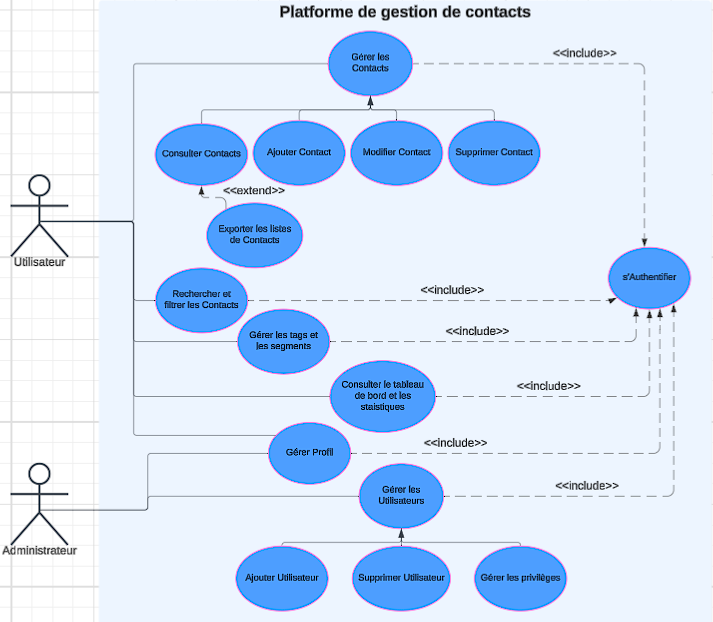
\includegraphics[width=0.6\textwidth]{images/diagramme_cas_utilisation.png}
\caption{Diagramme de cas d'utilisation du système}
\label{fig:dcu}
\end{figure}

Côté Utilisateur, les cas d'utilisation identifiés sont : s'authentifier, gérer son profil, gérer les contacts, exporter les listes, rechercher et filtrer, gérer les tags et les segments, et consulter le tableau de bord. L'Administrateur dispose d'un cas d'utilisation distinct, la gestion des comptes utilisateurs, sans accès aux fonctionnalités de l'Utilisateur.

\section{Besoins fonctionnels}

Les besoins fonctionnels précisent, pour chaque module, les fonctionnalités attendues de la plateforme. Ils sont présentés ci-dessous selon la logique de travail de l'application, puis résumés dans le tableau~\ref{tab:bf-synthese}.

\paragraph{Authentification et profil.}
Ce module sécurise l'accès à la plateforme : l'utilisateur s'authentifie par un identifiant et un mot de passe et peut gérer son profil.

\paragraph{Gestion des contacts.}
Ce module, au cœur de la plateforme, regroupe pour chaque contact des champs structurés (nom, organisation, pays, courriel).

\paragraph{Import.}
L'import alimente la base à partir de fichiers CSV ou Excel : les colonnes sont mises en correspondance, la validité des données est contrôlée et les doublons sont détectés, notamment par adresse électronique.

\paragraph{Numérisation OCR.}
La numérisation enrichit la base depuis des cartes de visite physiques : l'image est acquise, les informations extraites automatiquement, puis la fiche pré-remplie peut être corrigée avant enregistrement.

\paragraph{Recherche et segmentation.}
La recherche combine plusieurs critères (nom, pays, affiliation) pour retrouver rapidement un contact, tandis que la segmentation permet d'enregistrer et de réutiliser un ensemble de filtres afin de constituer des sous-ensembles de contacts.

\paragraph{Assistant IA.}
L'assistant permet d'interroger la base en langage naturel : les questions sont relayées à un service dédié qui consulte les contacts, en produit la synthèse et fournit des statistiques.

\paragraph{Tableau de bord.}
Le tableau de bord donne une vue de synthèse : des indicateurs récapitulent le nombre de contacts et leur répartition selon différents critères, avec une exploration interactive.

\paragraph{Export.}
L'export produit des fichiers CSV des listes de contacts, filtrées ou segmentées, avec la possibilité de personnaliser les champs inclus.

\paragraph{Administration.}
Ce module, réservé à l'administrateur, gouverne l'accès des utilisateurs à la plateforme par la gestion des comptes et l'attribution des rôles.

\begin{table}[H]
\centering
\small
\begin{tabularx}{\textwidth}{|l|X|}
\hline
\textbf{Module} & \textbf{Besoins clés} \\
\hline
Authentification et profil & Connexion et déconnexion sécurisées, gestion du profil, contrôle d'accès par rôle \\
\hline
Gestion des contacts & Création, consultation, modification et suppression des contacts (\acf{CRUD}), affichage de la liste \\
\hline
Import & Import CSV et Excel avec correspondance des colonnes, contrôle de validité des données, déduplication \\
\hline
Numérisation OCR & Acquisition d'une image de carte de visite, extraction automatique des informations, pré-remplissage et correction \\
\hline
Recherche et segmentation & Recherche multi-critères, filtrage, gestion des tags, segmentation \\
\hline
Assistant IA & Consultation de la base en langage naturel, synthèse d'un contact, statistiques \\
\hline
Tableau de bord & Indicateurs de synthèse, répartition des contacts par critères, exploration interactive \\
\hline
Export & Export des listes de contacts au format CSV, personnalisation des champs \\
\hline
Administration & Création et gestion des comptes utilisateurs, attribution des rôles, réservée à l'administrateur \\
\hline
\end{tabularx}
\caption{Besoins fonctionnels par module}
\label{tab:bf-synthese}
\end{table}

\section{Spécification des besoins non fonctionnels}

Outre les besoins fonctionnels, la plateforme doit satisfaire des exigences transverses de qualité, résumées dans le tableau~\ref{tab:bnf}.

\begin{table}[H]
\centering
\begin{tabularx}{\textwidth}{|l|l|X|}
\hline
\textbf{Catégorie} & \textbf{Besoin} & \textbf{Description} \\
\hline
Sécurité & Authentification et rôles & Accès sécurisé par mot de passe et contrôle d'accès par rôle \\
\hline
Sécurité & Protection des données & Accès aux contacts restreint aux utilisateurs authentifiés \\
\hline
Ergonomie & Interface conviviale & Interface web intuitive, responsive et facile à prendre en main \\
\hline
Performance & Temps de réponse & Réponses aux opérations courantes dans des délais acceptables \\
\hline
Maintenabilité & Architecture modulaire & Séparation claire des couches pour faciliter l'évolution \\
\hline
Déploiement & Disponibilité & Déploiement sur une infrastructure cloud accessible en ligne \\
\hline
\end{tabularx}
\caption{Besoins non fonctionnels}
\label{tab:bnf}
\end{table}
